% SCOPAS dual-layer revision of the UTM / MUSCAT sensor-placement paper
% Target venue: IEEE/AIAA DASC (IEEEtran)

\documentclass[conference]{IEEEtran}

\usepackage{cite}
\usepackage{amsmath,amssymb,amsfonts}
\usepackage{algorithmic}
\usepackage{graphicx}
\usepackage{textcomp}
\usepackage{xcolor}
\usepackage{booktabs}
\usepackage{multirow}
\usepackage{url}
\usepackage{hyperref}

\newcommand{\mc}{M_c}
\newcommand{\mg}{M_g}
\newcommand{\mwp}{M_{wp}}
\newcommand{\pnet}{\bar{P}_{Net}}
\newcommand{\rnet}{\bar{R}}

\begin{document}

\title{Dual-Layer Multi-Objective Sensor Placement for Urban BVLOS Surveillance}

\author{
\IEEEauthorblockN{Your Name\IEEEauthorrefmark{1}, Co-Author Name\IEEEauthorrefmark{2}}
\IEEEauthorblockA{\IEEEauthorrefmark{1}Your Institution, Department\\
City, Country\\
Email: your.email@institution.edu}
\IEEEauthorblockA{\IEEEauthorrefmark{2}Co-Author Institution\\
Email: coauthor@institution.edu}
}

\maketitle

\begin{abstract}
Urban Beyond Visual Line of Sight (BVLOS) operations require Ground-Based Surveillance Systems (GBSS) that separately account for \emph{cooperative} traffic (e.g., Remote~ID / RF) and \emph{non-cooperative} dark targets (Radar, EO, Acoustic). Collapsing both into a single coverage score systematically understates dark-target risk. This paper revisits city-scale sensor placement with the SCOPAS dual-layer framework: multi-objective NSGA-II optimizing threat-weighted \(M_{wp,coop}\), \(M_{wp,noncoop}\), and CapEx (hardware + site activation) under 3D LoS occlusion, with Acoustic as a low-cost non-cooperative modality and explicit planning floors (e.g., \(0.90/0.35\)).

On a 1\,km$\times$1\,km synthetic city with five critical assets, a dual-layer front of 32 solutions spans cooperative coverage \(0.07\)--\(0.96\) and non-cooperative coverage \(0.00\)--\(0.56\). Cooperative \(\geq90\%\) is reachable near \$247k, yet the same plans leave non-cooperative coverage near \(0.13\); joint floors near \(0.85/0.35\) cost about \$320k, while a strict \(0.90/0.50\) box remains a stretch. Airway-stratified maps retain the altitude-gap finding of prior work. Complementary airport split fronts and requirement-seeking demos reinforce the operational claim: BVLOS infrastructure cases must report cooperative and non-cooperative sensing fronts separately, and select deployments from dual-layer Pareto sets rather than a single fused score.
\end{abstract}

\begin{IEEEkeywords}
Beyond Visual Line of Sight (BVLOS), Urban Air Mobility (UAM), Ground-Based Surveillance Systems (GBSS), Dual-layer sensing, Counter-UAS, Multi-sensor optimization, NSGA-II, Acoustic sensing, OpenStreetMap
\end{IEEEkeywords}

\section{Introduction}

\subsection{Enabling Safe BVLOS and UAM Operations}

The rapid expansion of Beyond Visual Line of Sight (BVLOS) drone operations and Urban Air Mobility (UAM) promises transformative economic and societal benefits, ranging from autonomous parcel delivery to passenger air taxis \cite{faa2023uam}. However, safe integration into dense urban airspace requires overcoming critical infrastructure challenges. Central among these is continuous, reliable surveillance coverage to support Detect-and-Avoid (DAA) capabilities for both manned and unmanned aircraft \cite{mueller2017enabling}.

Current manned air traffic relies on cooperative transponders and centralized Air Traffic Control (ATC), but BVLOS/UAM operations introduce uncooperative airspace users—malfunctioning drones, hobbyist UAVs, or unauthorized vehicles—that must still be detected to prevent collisions and ensure public safety \cite{faa2020utm}. The resulting surveillance uncertainty directly limits airspace capacity: regulators may mandate conservative separation minima (e.g., 500 m radius) when detection reliability is low, whereas high-confidence monitoring can reduce separations by an order of magnitude \cite{nasa2021utm}. This makes surveillance infrastructure a critical enabler of operational scalability for urban air corridors.

\subsection{Ground-Based Surveillance Systems (GBSS)}

Ground-Based Surveillance Systems (GBSS) provide the foundational monitoring layer for UTM, complementing onboard DAA sensors with persistent infrastructure-supported detection \cite{kopardekar2016unmanned}. Multiple sensor modalities are employed, each with trade-offs:

\begin{itemize}
    \item \textbf{Radar}: robust in adverse weather and all lighting conditions, but limited in detecting small radar cross-section (RCS) UAVs at longer distances \cite{guvenc2018detection,semkin2020analyzing}.
    
    \item \textbf{RF/RID Receivers}: cost-effective and low-power, but dependent on cooperative transmitters \cite{guvenc2018detection,besada2022cuas}.
    
    \item \textbf{Electro-Optical/Infrared (EO/IR) sensors}: high-resolution visual coverage, but degraded by fog, rain, or night conditions \cite{guvenc2018detection,yan2023passive}.
    
    \item \textbf{Acoustic sensors}: can detect propeller noise without line-of-sight, but are highly susceptible to urban background noise \cite{guvenc2018detection,yan2023passive}.
\end{itemize}

This diversity motivates heterogeneous multi-sensor networks, combining complementary modalities to ensure robust coverage and redundancy, as emphasized in counter-UAS and UTM surveillance literature \cite{muscat2023,besada2022cuas,blasch2021information}. Despite significant interest, designing cost-effective GBSS remains challenging: one must optimize the number, type, and placement of sensors over large urban areas, balancing coverage, redundancy, and budget while considering deployment constraints such as rooftop accessibility, line-of-sight obstructions, and regulatory limits \cite{aievola2022ground,dulia2024sand}.

\subsection{Prior Work on Sensor Placement Optimization}

Several frameworks have addressed GBSS or C-UAS sensor allocation (detailed comparison in Section~\ref{sec:related}, Table~\ref{tab:related_comparison}):

\textbf{MUSCAT} \cite{muscat2023}: multi-sensor C-UAS placement with coverage/gap/cost metrics and exhaustive search over elevation-oriented terrain models. Rigorous for small candidate sets, but $O(2^n)$ search is intractable beyond roughly 10--15 locations.

\textbf{Radar / AAM network design}: Aievola et al.\ analyze ground-based radar networks for UAM \cite{aievola2022ground}; Dulia and Shihab optimize AAM surveillance networks under cost and detection-probability floors over terrain classes \cite{dulia2024sand}. These advance placement for cooperative/non-cooperative AAM traffic but do not jointly expose dual-layer OSM+ray-trace CapEx Pareto fronts of the form pursued here.

\textbf{Metaheuristics}: NSGA-II and related MOEAs are standard for coverage--cost placement in WSN and radar management \cite{deb2002fast,molina2008layout,iqbal2015wsn,charlish2016radar}, motivating transfer to occlusion-aware GBSS chromosomes.

\subsection{Remaining Challenges}

Despite progress, three gaps persist in urban GBSS design (Table~\ref{tab:related_comparison}):

\textbf{Scalability}: Exhaustive and many MIP formulations become impractical for tens of heterogeneous sensors across square kilometers with occlusion physics \cite{muscat2023,katoh1998resource}.

\textbf{Urban Environment Fidelity}: Statistical LoS models omit building-resolved shadowing that dominates low airways \cite{3gpp38901,itur_p1411}; OSM-enabled deterministic LoS for C-UAS CapEx planning remains comparatively sparse relative to telecom uses of OSM \cite{osm_applications}.

\textbf{Operational Metric Split}: Cooperative RID/RF coverage and non-cooperative dark-target coverage are often collapsed into one score, understating dark-target risk for BVLOS safety cases \cite{besada2022cuas,blasch2021information}.

\subsection{Contributions}

This paper revises and extends prior city-scale GBSS optimization (MUSCAT / SCOPAS lineage) with a dual-layer operational framing and two claim-closing controls:

\begin{enumerate}
    \item \textbf{Dual-layer multi-objective placement}: NSGA-II optimizes threat-weighted \(M_{wp,coop}\) and \(M_{wp,noncoop}\) jointly with CapEx, instead of a single fused coverage score.
    \item \textbf{Heterogeneous non-cooperative mix}: Radar, EO, and Acoustic form the dark-target layer; RF is cooperative-only. Acoustic provides a documented low-CapEx non-coop filler---without claiming universal heterogeneity dominance on classic \(M_c\).
    \item \textbf{Requirement floors for planning}: Explicit joint corridors (e.g., \(0.90/0.35\)) with Pareto filtering replace opaque GREEN thresholds and unsupported ``\% of optimum'' claims.
    \item \textbf{Evidence across scenes}: Synthetic city asset-weighted fronts, airport split coop/noncoop runs, and short target-seeking demos quantify the coop-cheap / noncoop-hard asymmetry for BVLOS safety cases.
    \item \textbf{Claim-closing controls}: (A)~small-$n$ oracle comparison (Exhaustive / Greedy / Random / GA) under the same ray-tracer; (B)~matched-budget classic \(M_c\) modality ablation; (C)~dual-layer CapEx ablation on \(M_{wp,coop}/M_{wp,noncoop}\). Together these bound GA gaps where enumeration is feasible and show when heterogeneity helps (joint dark-target floors) versus when RF-only wins (lean classic/coop coverage).
\end{enumerate}

Locked contribution sentence: NSGA-II with deterministic 3D ray-tracing and OSM geometry yields dual-layer GBSS Pareto fronts spanning cooperative \(M_{wp}\) near \(0.07\)--\(0.96\) and non-cooperative \(M_{wp}\) near \(0.00\)--\(0.56\) on a synthetic city (with complementary airport and Paulista lite fronts), in a \(g\cdot p\) evaluation regime where exhaustive MUSCAT search is intractable for \(n\gtrsim25\) sites; city-scale optimality gaps and universal heterogeneity dominance remain unsupported.

The remainder of this paper is organized as follows: Section II reviews related work and the systems comparison table. Section III formulates the dual-layer problem. Section IV--V describe methodology and SCOPAS implementation. Section VI presents experimental setup. Section VII analyzes dual-layer results and Controls~A--C. Section VIII discusses implications and limits. Section IX concludes.


% Section 2: Related Work (strengthened literature review)

\section{Related Work}
\label{sec:related}

We organize prior art along four streams that frame GBSS planning for BVLOS: (i)~multi-sensor C-UAS / UTM sensing, (ii)~surveillance network \emph{placement} for UAM/AAM, (iii)~multi-objective / metaheuristic placement methods, and (iv)~urban LoS geometry. Table~\ref{tab:related_comparison} summarizes closest systems work against this paper's dual-layer SCOPAS framing.

\begin{table*}[t]
\centering
\caption{Systems comparison of closely related GBSS / C-UAS / AAM surveillance placement work and method analogs. Tokens summarize scope; ``---'' means not the paper's focus.}
\label{tab:related_comparison}
\setlength{\tabcolsep}{3pt}
\begin{tabular}{lccccccc}
\toprule
\textbf{Work} & \textbf{Sensors} & \textbf{Urban geometry / LoS} & \textbf{Objectives} & \textbf{Optimizer} & \textbf{Coop$\neq$Noncoop} & \textbf{City-scale case} \\
\midrule
Guvenc et al.\ \cite{guvenc2018detection} & Multi (survey) & --- & Detection/tracking & --- & Partial & --- \\
Besada et al.\ \cite{besada2022cuas} & Radar/RF/EO/Ac & Sim.\ models & C-UAS for UTM & --- & Yes (noncollab.) & --- \\
Yan et al.\ \cite{yan2023passive} & RF/Ac/vision & Urban survey & Detection/tracking & --- & Implicit & --- \\
MUSCAT \cite{muscat2023} & Heterogeneous & DTED / elev. & $M_c$, $M_g$, cost & Exhaustive & No (fused) & Small / synthetic \\
Aievola et al.\ \cite{aievola2022ground} & Radar & Urban UAM & Coverage / radar net & MIP / analysis & No & Corridor-scale \\
Dulia \& Shihab (SAND) \cite{dulia2024sand} & Multi-type AAM & Terrain classes & Cost + $P_D$ floors & ILP / design & Discussed & Multi-city OH \\
Molina et al.\ \cite{molina2008layout} & Homog.\ WSN & Flat field & Nodes + energy & NSGA-II / MOEA & --- & Synthetic field \\
Iqbal et al.\ \cite{iqbal2015wsn} & WSN (survey) & --- & Coverage/cost/\ldots & MOEA survey & --- & --- \\
Charlish et al.\ \cite{charlish2016radar} & Radar & --- & Sensor management & GA & --- & --- \\
\textbf{This work} & Radar+RF+EO+Ac & OSM + ray-trace & $M_{wp,\mathrm{coop}}$, $M_{wp,\mathrm{noncoop}}$, CapEx & NSGA-II & \textbf{Yes} & City + SJC + Paulista lite \\
\bottomrule
\end{tabular}
\end{table*}


\subsection{Multi-Sensor C-UAS Sensing for UTM}

Amateur and small-UAV detection surveys emphasize complementary modalities---radar, RF/Remote~ID, EO/IR, and acoustic---and the value of fusion under urban clutter \cite{guvenc2018detection,yan2023passive}. Multisensor track fusion can maintain tracks under partial sensor outages \cite{jovanoska2018multisensor,dudczyk2022multisensor}, while small-RCS phenomenology remains challenging for radar alone \cite{semkin2020analyzing}. For UTM specifically, Besada et al.\ review Counter-UAS sensors and provide simulation models for noncollaborative surveillance feeding tactical UTM services \cite{besada2022cuas}. Blasch et al.\ argue that information fusion is an autonomy enabler for UTM \cite{blasch2021information}, consistent with classical JDL-style fusion handbooks \cite{liggins2009handbook}.

These works establish \emph{why} heterogeneous GBSS matter and that cooperative (e.g., RID/RF) and non-cooperative (radar/EO/acoustic) sensing address different threat classes. They typically stop at detection algorithms, sensor models, or system architecture---not CapEx-constrained placement under city-scale LoS occlusion with separate coop/noncoop coverage objectives.

\subsection{Surveillance Network Placement for UAM / AAM}

Closest placement literature includes MUSCAT, which formulates multi-sensor C-UAS placement with coverage/gap/cost metrics and exhaustive search over candidate sites, adopting elevation-oriented terrain models \cite{muscat2023}. Exhaustive enumeration guarantees small-$n$ optima but becomes intractable beyond roughly 10--15 sites. Aievola et al.\ study ground-based radar networks for UAM with design and performance analysis under urban constraints, leaning on mathematical programming / structured radar-network design rather than multi-modal CapEx Pareto fronts \cite{aievola2022ground}. Dulia and Shihab's SAND model designs AAM surveillance networks that minimize sensor cost subject to coverage and detection-probability floors over terrain classes, and discusses cooperative vs.\ non-cooperative sensing options in a cost--benefit setting \cite{dulia2024sand}. Resource-allocation MIP surveys underline scalability limits once formulations become non-convex \cite{katoh1998resource}.

Relative to these, our work keeps MUSCAT's metric lineage and heterogeneous mix, but (i)~optimizes threat-weighted \emph{dual-layer} $M_{wp,\mathrm{coop}}$ and $M_{wp,\mathrm{noncoop}}$ jointly with CapEx via NSGA-II, (ii)~uses OSM building geometry with deterministic ray-traced LoS, and (iii)~reports city/airport/Paulista fronts plus matched CapEx ablations (Controls~B--C) rather than a single fused score or exhaustive optimum claim.

\subsection{Multi-Objective and Metaheuristic Placement}

Holland's GA foundations \cite{holland1992adaptation} and Deb's NSGA-II \cite{deb2002fast} underpin Pareto search for discrete placement. WSN layout has long used MOEAs to trade coverage, node count, and energy \cite{molina2008layout,iqbal2015wsn,zou2019WSN}; radar sensor management has likewise used GAs \cite{charlish2016radar}. We treat these as \emph{method transfer}: coverage--cost Pareto search is mature in WSN/radar management, but transferring it to urban C-UAS GBSS requires occlusion-aware $P_D$ models and an explicit coop/noncoop objective split that WSN energy/connectivity formulations do not provide.

\subsection{Urban Geometry and Line-of-Sight Modeling}

Statistical urban channel models (e.g., 3GPP TR~38.901 LoS probability) and ITU short-range outdoor recommendations support radio planning without full building footprints \cite{3gpp38901,itur_p1411}. OpenStreetMap provides globally available building footprints used across geospatial and telecom studies \cite{osm_applications,elias2023exploring}. Deterministic ray-tracing on voxelized OSM buildings is more conservative than statistical LoS and yields altitude-stratified shadow zones---the geometry regime we adopt for GBSS planning.

\subsection{Gap Analysis}

Table~\ref{tab:related_comparison} highlights three persistent gaps: (1)~placement papers rarely expose \emph{separate} cooperative and non-cooperative coverage objectives under CapEx; (2)~exhaustive / MIP approaches struggle at city-scale candidate sets with heterogeneous types and occlusion physics; (3)~urban C-UAS placement validations seldom combine OSM geometry, ray-traced LoS, and multi-city (or multi-scene) Pareto evidence. This paper addresses (1)--(3) within a $g\cdot p$ NSGA-II budget, with Controls~A--C bounding small-$n$ quality and CapEx-matched modality claims---without asserting city-scale optimality gaps.

\input{sections/03_problem_formulation}
% Section 4: Methodology

\section{Enhanced MUSCAT Methodology}

Our methodology extends the four-phase MUSCAT approach with three key enhancements: GA-based optimization, OSM urban environment integration, and deterministic ray-tracing.

\subsection{Phase 1: Environment Setup}

\subsubsection{Urban Data Acquisition}

Unlike MUSCAT's terrain-focused approach using DTED maps \cite{muscat2023}, we employ OpenStreetMap (OSM) to obtain real urban building footprints \cite{osm_applications,elias2023exploring}:

\begin{algorithmic}
\STATE Input: Latitude, Longitude, Radius
\STATE Download buildings from OSM API
\STATE Extract geometries (Polygon/MultiPolygon)
\STATE Estimate heights (from metadata or heuristics)
\STATE Reproject to UTM coordinates (meters)
\STATE Translate to local origin
\STATE Output: Buildings GeoJSON
\end{algorithmic}

This approach enables analysis of any urban area worldwide with freely available, crowd-sourced data that includes building footprints and attributes.

\subsubsection{3D Voxelization}

We discretize the urban environment into a 3D occupancy grid:

\begin{equation}
\text{Grid}(i,j,k) = \begin{cases}
1 & \text{if voxel occupied by building} \\
0 & \text{if free space}
\end{cases}
\end{equation}

where $(i,j,k)$ are voxel indices and resolution $r$ (typically 10-20m) is user-configurable. This voxelization enables efficient ray-tracing and LoS calculations.

\subsection{Phase 2: Sensor Attributes and ROI Definition}

\subsubsection{Sensor Models with Field-of-View Constraints}

We implement four sensor types with realistic Field-of-View (FOV) parameters:

\textbf{Radar}: Active sensor with 360° horizontal coverage and limited elevation:
\begin{equation}
P_D^{radar} = \begin{cases}
f(P_t, G, \sigma_{RCS}, R, \lambda) & \text{if } \theta_{elev} \in [-5°, 30°] \\
0 & \text{otherwise}
\end{cases}
\end{equation}
where $\theta_{elev}$ is the elevation angle from sensor to target.

\textbf{RF Passive (RID equivalent)}: Nearly omnidirectional ($\theta_{elev} \in [-30°, 70°]$):
\begin{equation}
P_D^{RF} = f(ERP, Sensitivity, R)
\end{equation}

\textbf{Electro-Optical (EO)}: Limited FOV (90° horizontal, $\theta_{elev} \in [-20°, 45°]$)

\textbf{Acoustic}: Omnidirectional ($\theta_{elev} \in [-40°, 80°]$)

These FOV constraints prevent unrealistic scenarios where rooftop sensors "see" targets far below horizon, improving model fidelity.

\subsubsection{Sensor Location Generation}

For real scenarios, sensor locations are automatically generated on a grid pattern while avoiding building interiors:

\begin{algorithmic}
\STATE Generate grid with spacing $s$ meters
\FOR{each grid point $(x, y)$}
  \IF{point not inside any building}
    \STATE Add location with height $h \sim U(25, 35)$ m
  \ENDIF
\ENDFOR
\end{algorithmic}

\subsection{Phase 3: Coverage Computation with Airway-Specific Analysis}

\subsubsection{Deterministic Ray-Tracing}

We replace statistical LoS probability models \cite{3gpp38901,itur_p1411} with deterministic ray-tracing on the voxelized building occupancy grid:

\begin{algorithmic}
\STATE Input: Sensor location $\mathbf{s}$, Target location $\mathbf{t}$
\STATE Calculate elevation angle $\theta_{elev} = \arctan\left(\frac{z_t - z_s}{\sqrt{(x_t-x_s)^2 + (y_t-y_s)^2}}\right)$
\IF{$\theta_{elev} \notin [\theta_{min}, \theta_{max}]$}
  \STATE $P_D = 0.0$ (outside FOV)
  \RETURN
\ENDIF
\STATE Discretize 3D line between $\mathbf{s}$ and $\mathbf{t}$
\STATE Sample voxels along the ray
\IF{any voxel is occupied}
  \STATE $P_{LoS} = 0.0$ (blocked)
\ELSE
  \STATE $P_{LoS} = 1.0$ (clear)
\ENDIF
\end{algorithmic}

This provides exact LoS determination with FOV constraints, improving model fidelity for urban scenarios where sensors are mounted on rooftops.

\subsubsection{Multi-Altitude Airway Analysis}

Urban airspace operations span multiple altitude layers. We evaluate coverage separately for three representative airways:

\begin{itemize}
\item \textbf{Low Airway (20m)}: Between buildings, high occlusion
\item \textbf{Medium Airway (45m)}: Above low-rise buildings, optimal for surveillance
\item \textbf{High Airway (65m)}: Above most buildings, clear line-of-sight
\end{itemize}

For each airway at altitude $h$, coverage is calculated excluding building-occupied volumes:

\begin{equation}
M_c^{(h)} = \frac{\sum_{(x,y) \in \text{Free}(h)} \mathbb{1}[\pnet(x,y,h) \geq \tau]}{|\text{Free}(h)|}
\label{eq:mc_airway}
\end{equation}

where $\text{Free}(h) = \{(x,y) : \text{Grid}(x,y,h) = 0\}$ is the set of unoccupied voxels at altitude $h$. This airway-specific analysis reveals altitude-dependent surveillance quality—critical for establishing BVLOS operational envelopes.

\subsubsection{Network Detection Probability}

For multiple sensors, we employ soft voting fusion:

\begin{equation}
\pnet = 1 - \prod_{i=1}^{N_s} (1 - P_{D,i})
\label{eq:pnet}
\end{equation}

where $P_{D,i}$ is the detection probability of the $i$-th sensor.

\subsubsection{Redundancy Metric}

System redundancy is calculated as:

\begin{equation}
\rnet = \frac{1}{N_{free}} \sum_{(i,j,k) \in \text{Free}} \frac{\sum_s P_{D,s}(i,j,k)}{N_s}
\label{eq:redundancy}
\end{equation}

where $N_{free}$ is the number of unoccupied voxels and $N_s$ is the number of active sensors.

\subsection{Phase 4: Genetic Algorithm Optimization}

\subsubsection{GA Implementation}

We employ DEAP (Distributed Evolutionary Algorithms in Python) \cite{deap2012} with the following operators:

\textbf{Selection}: Tournament selection with tournament size 3

\textbf{Crossover}: Two-point crossover preserving gene structure

\textbf{Mutation}: 
\begin{itemize}
\item Location mutation: Change $l_i$ to random valid location
\item Type mutation: Change $t_i$ to different sensor type
\item Activation mutation: Toggle $a_i$ between 0 and 1
\end{itemize}

\textbf{Fitness Evaluation}: Equation \ref{eq:fitness} with parallelized computation across available CPU cores.

\subsubsection{Convergence and Elitism}

We maintain the best individual across generations (elitism) and track fitness statistics to monitor convergence. Typical runs achieve stable solutions within 50-100 generations for population sizes of 30-50.

\subsection{Multi-Objective Optimization with NSGA-II}

The sensor placement problem inherently involves conflicting objectives that cannot be simultaneously optimized. To address this, we employ the Non-dominated Sorting Genetic Algorithm II (NSGA-II) \cite{deb2002fast}, following the multi-objective placement tradition in WSN/radar management \cite{molina2008layout,iqbal2015wsn,charlish2016radar} but with dual-layer GBSS objectives. In the dual-layer SCOPAS configuration the primary objectives are threat-weighted $M_{wp,\mathrm{coop}}$, $M_{wp,\mathrm{noncoop}}$, and CapEx (maximize, maximize, minimize); the classical $M_c$/redundancy/cost triple below documents the MUSCAT-compatible scalarized lineage.

\subsubsection{Problem Formulation}

Given a sensor configuration $X$, we define three objectives:

\begin{align}
\text{maximize} \quad & f_1(X) = M_c(X) \quad \text{(Coverage Index)} \label{eq:obj1}\\
\text{maximize} \quad & f_2(X) = \bar{R}(X) \quad \text{(Mean Redundancy)} \label{eq:obj2}\\
\text{minimize} \quad & f_3(X) = C(X) \quad \text{(Total Cost)} \label{eq:obj3}
\end{align}

A solution $X_1$ \textit{dominates} $X_2$ if $X_1$ is no worse in all objectives and strictly better in at least one. The \textit{Pareto-optimal front} is the set of all non-dominated solutions.

\subsubsection{NSGA-II Algorithm}

NSGA-II discovers the Pareto front through:

\begin{enumerate}
\item \textbf{Non-dominated Sorting}: Population is partitioned into fronts $F_1, F_2, \ldots$ where $F_1$ contains all non-dominated individuals, $F_2$ contains individuals dominated only by $F_1$, etc.

\item \textbf{Crowding Distance}: Within each front, individuals are assigned a crowding distance measuring solution density. Larger distances indicate less crowded regions, promoting solution diversity along the Pareto front.

\item \textbf{Selection}: Tournament selection favors individuals with better (lower) front rank and, for equal rank, larger crowding distance—balancing convergence toward Pareto front with diversity maintenance.

\item \textbf{Elitism}: The best non-dominated solutions are preserved across generations, ensuring Pareto front quality monotonically improves.
\end{enumerate}

This approach provides decision-makers with a continuum of optimal trade-offs rather than a single prescribed configuration, enabling context-specific infrastructure selection based on operational requirements, budget constraints, and risk tolerance.

\subsection{Computational Complexity Analysis}

\textbf{MUSCAT Exhaustive Search}:
\begin{equation}
O(\text{MUSCAT}) = O\left(\sum_{k=1}^{n} \binom{n}{k}\right) = O(2^n)
\end{equation}

\textbf{Our GA Approach}:
\begin{equation}
O(\text{GA}) = O(g \cdot p \cdot e)
\end{equation}
where $g$ is generations, $p$ is population size, and $e$ is evaluation complexity.

For $n=30$ locations:
\begin{itemize}
\item MUSCAT: $2^{30} \approx 10^9$ evaluations (intractable)
\item GA: $50 \times 30 \times e = 1,500 \cdot e$ evaluations (feasible)
\end{itemize}

This represents approximately 6 orders of magnitude reduction in computational requirements, enabling optimization of much larger networks.



\input{sections/05_implementation}
% Section 6: Experimental Setup (SCOPAS dual-layer revision)

\section{Experimental Setup}
\label{sec:setup}

All experiments use the open SCOPAS framework (Radar, RF, EO, Acoustic) with dual-layer NSGA-II objectives \((M_{wp,coop}, M_{wp,noncoop}, \mathrm{cost})\) unless a split profile is stated. Sensor CapEx defaults: Radar \$50k, RF \$15k, EO \$25k, Acoustic \$8k, plus site activation \$15k.

\subsection{Synthetic city}

Scene: 1\,km$\times$1\,km, 196 buildings, 221 candidate sites (\texttt{data/examples/city\_10x10\_*}). Five critical assets define the threat map. Airway altitudes \(\{20,45,65\}\)\,m. Cloud-feasible paper rerun: resolution 30\,m, population 32, 18 generations, 4 cores (\texttt{configs/paper\_rerun\_city\_dual.json}).

Planning floors used for post-filtering: \(M_{wp,coop}\geq0.90\), \(M_{wp,noncoop}\geq0.35\) (practical) and stretch \(0.90/0.50\).

\subsection{Airport SJC (split fronts)}

Real OSM airport scene with runway exclusion. Split optimization runs \texttt{coop\_only} then \texttt{noncoop\_only} (\texttt{--split-objectives}) so dark-target cost is not hidden inside a cooperative optimum. Lite paper budget: resolution 40\,m, population 24, 12 generations.

\subsection{Avenida Paulista (lite)}

Real corridor scene retained for continuity with the prior draft, executed at reduced fidelity (resolution 40\,m, smaller GA) for cloud reproducibility. Full 80$\times$45 @ 20\,m remains a longer checkpointed job.

\subsection{Analysis pipeline}

Each run emits Pareto JSON, hypervolume, convergence plots, LoS-aware overview maps, flight-level \(M_c\), and cost-vs-threshold curves. Dual-layer fronts additionally emit coop$\times$noncoop target plots; \texttt{tools/select\_requirement\_solutions.py} reports cheapest feasible members under stated floors.

% Section 7: Results (SCOPAS dual-layer revision)
% Numbers below are from paper_rerun_city_dual / run_medium (see MANIFEST.md).
% Replace airport / Paulista placeholders once those runs complete.

\section{Results and Analysis}
\label{sec:results}

We report dual-layer NSGA-II fronts under SCOPAS: maximize threat-weighted cooperative coverage \(M_{wp,coop}\) and non-cooperative coverage \(M_{wp,noncoop}\) while minimizing CapEx (hardware + site activation). Non-cooperative sensors are Radar, EO, and Acoustic; RF contributes only to the cooperative layer.

\subsection{Synthetic city (1\,km$\times$1\,km, five critical assets)}

Configuration: resolution 30\,m, population 32, 18 generations, 4 cores, sensor budget 3--15, Acoustic enabled. The run produced 32 non-dominated solutions. Cooperative coverage spans \(0.074\)--\(0.963\); non-cooperative coverage spans \(0.003\)--\(0.563\).

\begin{figure}[t]
  \centering
  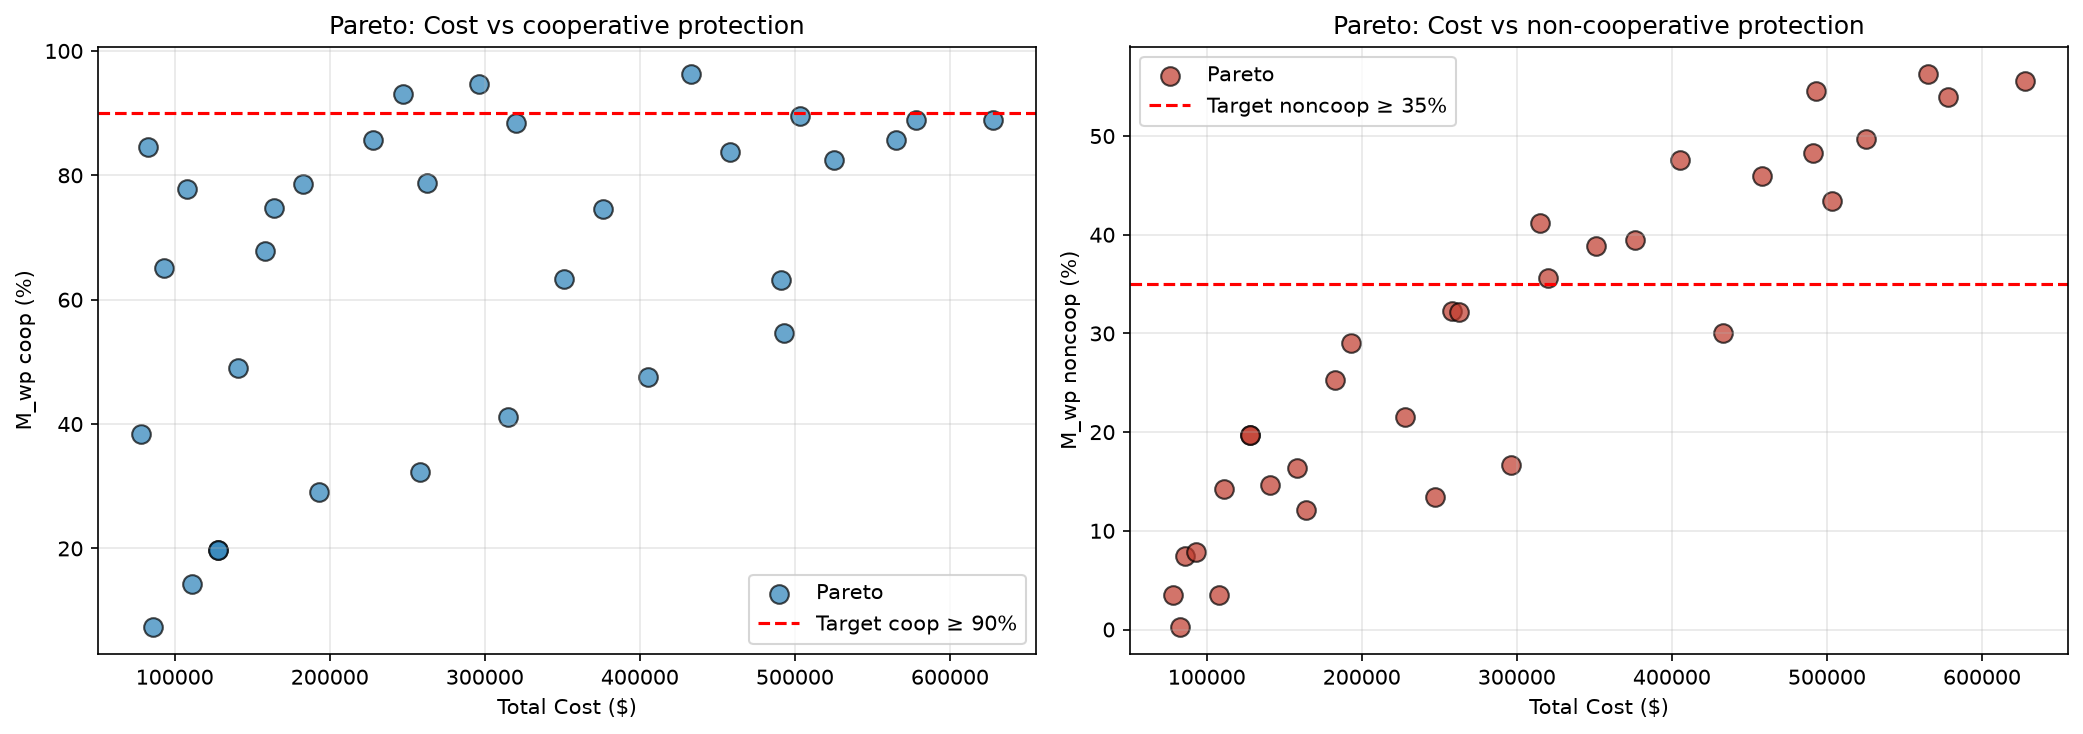
\includegraphics[width=0.48\textwidth]{figures/scopas/city_pareto_front.png}
  \caption{Dual-layer Pareto projections for the synthetic city (cost vs.\ \(M_{wp,coop}\) and \(M_{wp,noncoop}\)).}
  \label{fig:city_pareto}
\end{figure}

\begin{figure}[t]
  \centering
  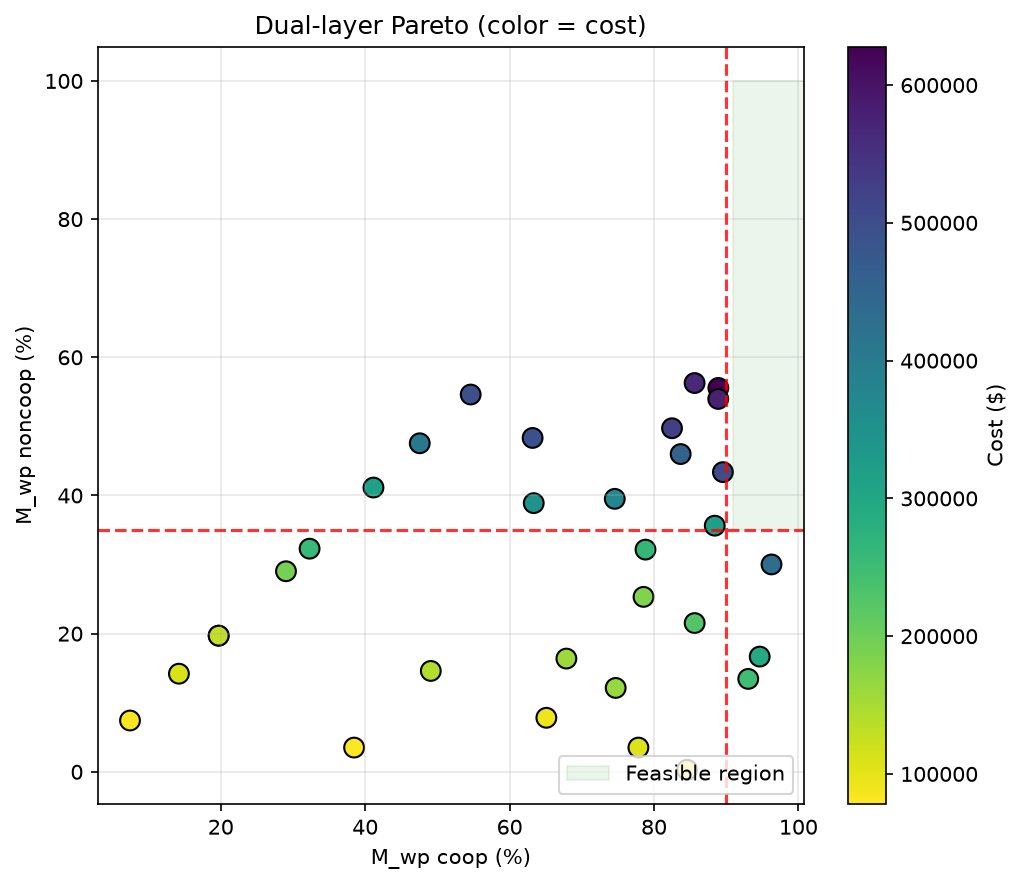
\includegraphics[width=0.48\textwidth]{figures/scopas/city_dual_targets.png}
  \caption{Coop$\times$noncoop trade space with planning floors \(M_{wp,coop}\geq0.90\) and \(M_{wp,noncoop}\geq0.35\) (green box). Color encodes CapEx.}
  \label{fig:city_targets}
\end{figure}

\subsubsection{Representative operating points}

\begin{table}[h]
\centering
\caption{Representative dual-layer solutions — synthetic city (SCOPAS rerun).}
\label{tab:city_dual}
\begin{tabular}{lcccc}
\toprule
\textbf{Regime} & \textbf{Mix} & \(M_{wp,coop}\) & \(M_{wp,noncoop}\) & \textbf{Cost} \\
\midrule
Cheap coop & 2RF+1Ac & 0.846 & 0.003 & \$83k \\
Joint near-floor & 4Rad+2RF & 0.884 & 0.356 & \$320k \\
High coop & 4Rad+5RF+1Ac & 0.963 & 0.300 & \$433k \\
Best joint miss & 6Rad+3RF+1Ac & 0.895 & 0.434 & \$503k \\
Best noncoop & 7Rad+2EO+1RF & 0.856 & 0.563 & \$565k \\
\bottomrule
\end{tabular}
\end{table}

\textbf{Finding 1 (layer asymmetry).}
Cooperative coverage \(\geq90\%\) is reachable near \$247k, but that individual only achieves \(M_{wp,noncoop}=0.134\). Dark-target coverage above \(0.50\) requires Radar-heavy mixes above \$500k and still does not jointly clear a strict \(0.90/0.50\) box in this budget.

\textbf{Finding 2 (practical joint floor).}
Under floors \(0.90/0.35\), the front has no feasible member (closest: \(0.895/0.434\) at \$503k). Softening to \(0.85/0.35\) yields five feasible solutions; cheapest \$320k (4 Radar + 2 RF). Stretch demos on the same geometry previously found a joint \(0.90/0.35\) solution at \$315k with a larger dual-layer search (see \texttt{demo\_targets} package).

\textbf{Finding 3 (altitude still matters).}
Flight-level analysis preserves the airway gap narrative: low airways remain occlusion-limited even when aggregate \(M_{wp}\) is high (Figure~\ref{fig:city_flight}).

\begin{figure}[t]
  \centering
  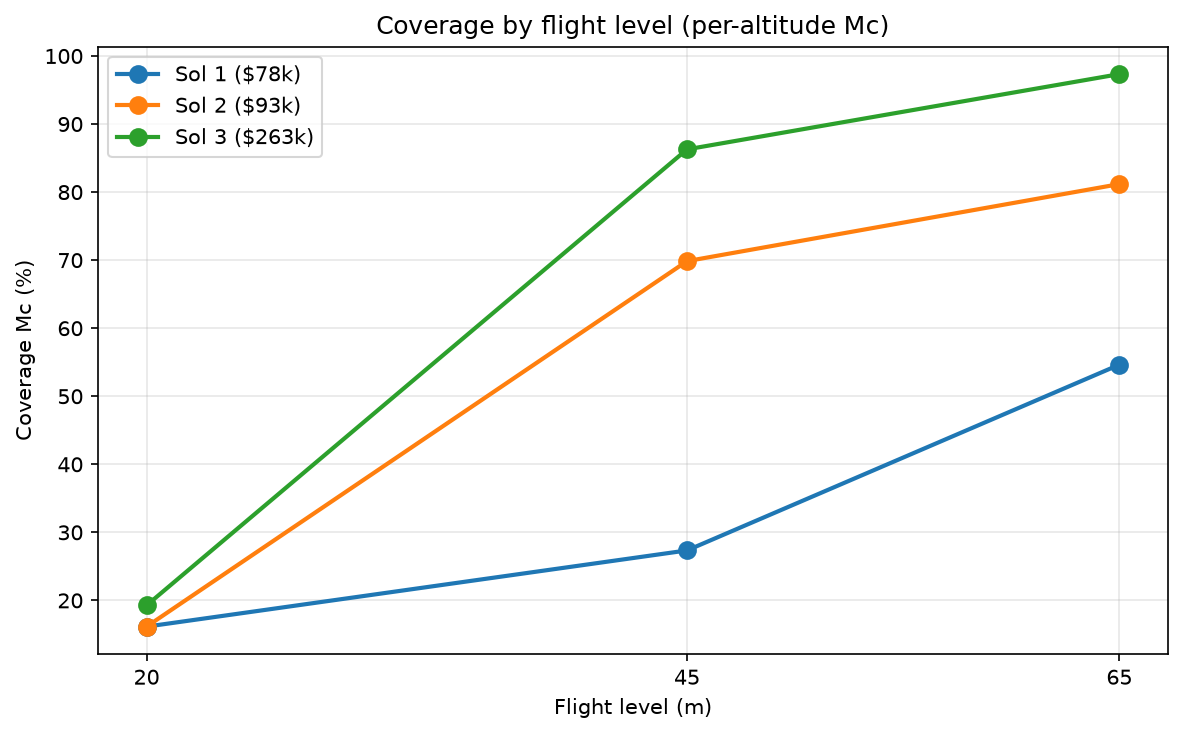
\includegraphics[width=0.48\textwidth]{figures/scopas/city_flight_levels.png}
  \caption{Coverage by flight level for representative Pareto members.}
  \label{fig:city_flight}
\end{figure}

\begin{figure}[t]
  \centering
  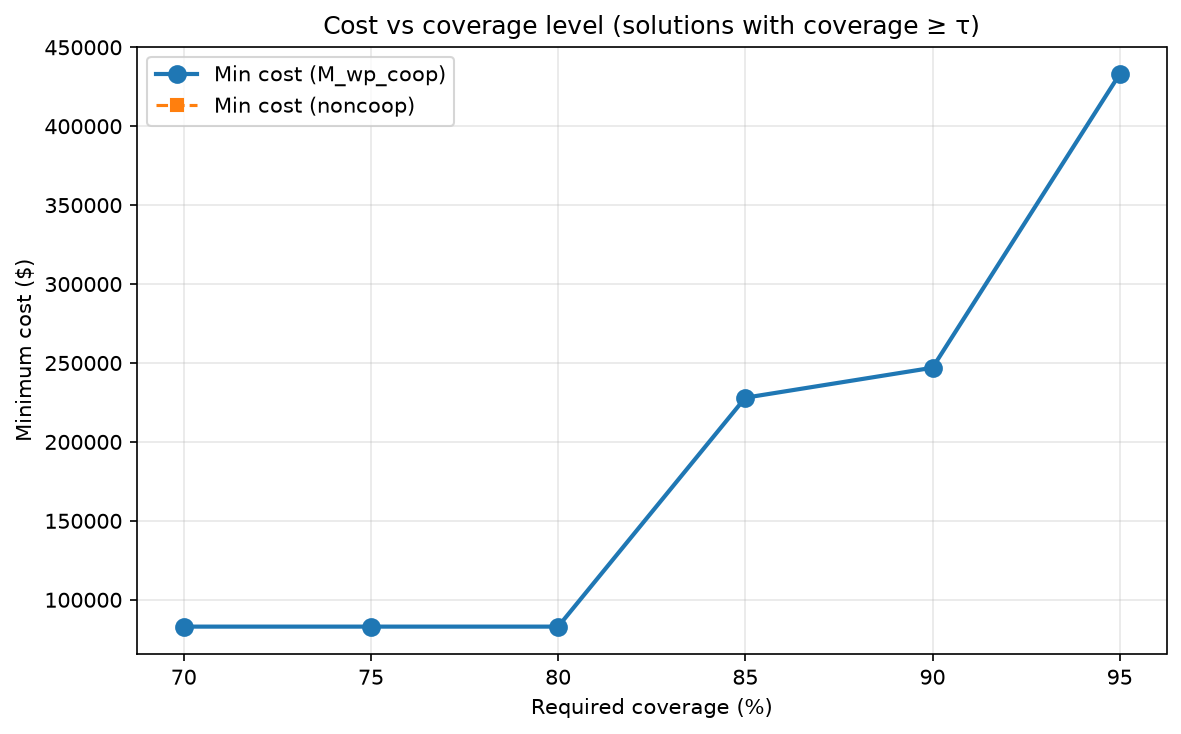
\includegraphics[width=0.48\textwidth]{figures/scopas/city_cost_vs_coverage.png}
  \caption{Minimum CapEx to reach cooperative \(M_{wp}\) thresholds; non-cooperative 70\%+ thresholds remain empty on this front.}
  \label{fig:city_cost_thr}
\end{figure}

\subsection{Requirement-seeking demos (prior short runs)}

Target-seeking configs aiming at \(0.90/0.35\) and stretch \(0.90/0.50\) confirm the same structure: cooperative floors are inexpensive with RF; joint dark-target floors near \(35\%\) are the practical planning corridor; \(50\%\) noncoop with \(\geq90\%\) coop remains a stretch (best observed joint near \(0.957/0.445\)).

\subsection{Airport SJC split fronts}

Split optimization on the São José dos Campos airport scene (resolution 40\,m, population 24, 12 generations) isolates each layer.

\textbf{Cooperative front.} Twenty-four solutions; \(M_{wp,coop}\) saturates to \(1.0\). The cheapest plan with \(M_{wp,coop}\geq0.90\) costs \$61k (1 RF + 2 Acoustic) but yields \(M_{wp,noncoop}\approx0.004\). High-coop RF-heavy plans at \$188k still leave non-cooperative coverage near zero.

\textbf{Non-cooperative front.} Twenty-four Radar/EO/Acoustic solutions span \(M_{wp,noncoop}\) from \(0.032\) to \(0.445\). Best observed dark-target coverage is \(0.445\) at \$405k (5 Radar + 2 EO); no plan reaches a 70\% noncoop threshold in this budget.

\begin{figure}[t]
  \centering
  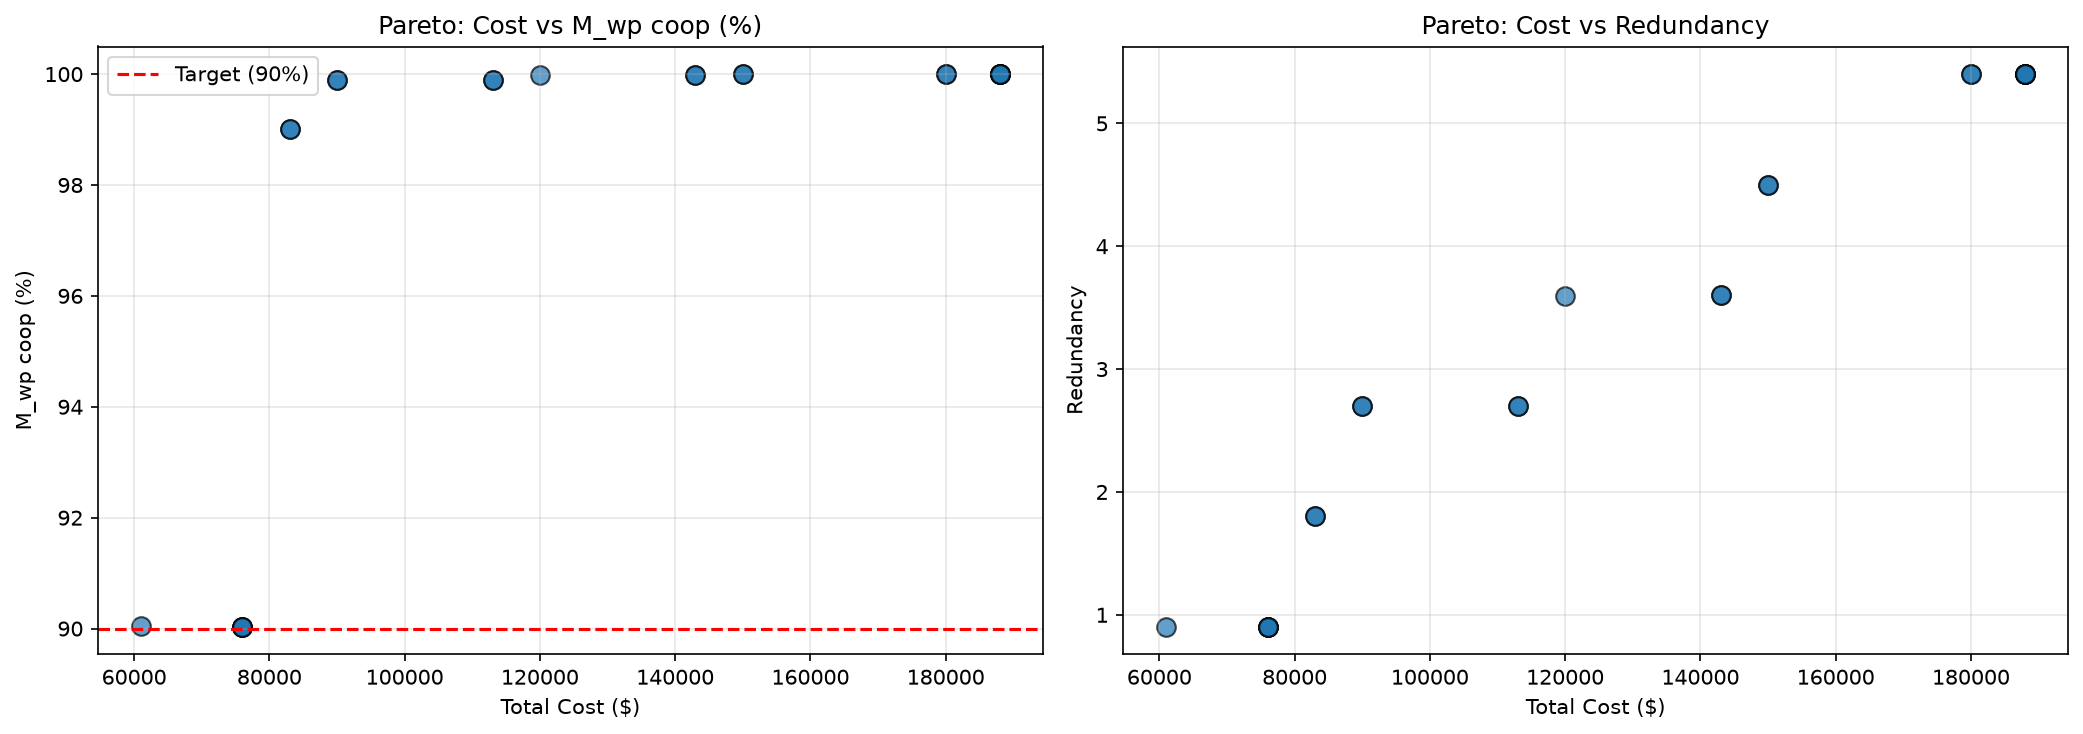
\includegraphics[width=0.48\textwidth]{figures/scopas/sjc_coop_pareto.png}
  \caption{Airport SJC cooperative-only Pareto (cost vs.\ \(M_{wp,coop}\)).}
  \label{fig:sjc_coop}
\end{figure}

\begin{figure}[t]
  \centering
  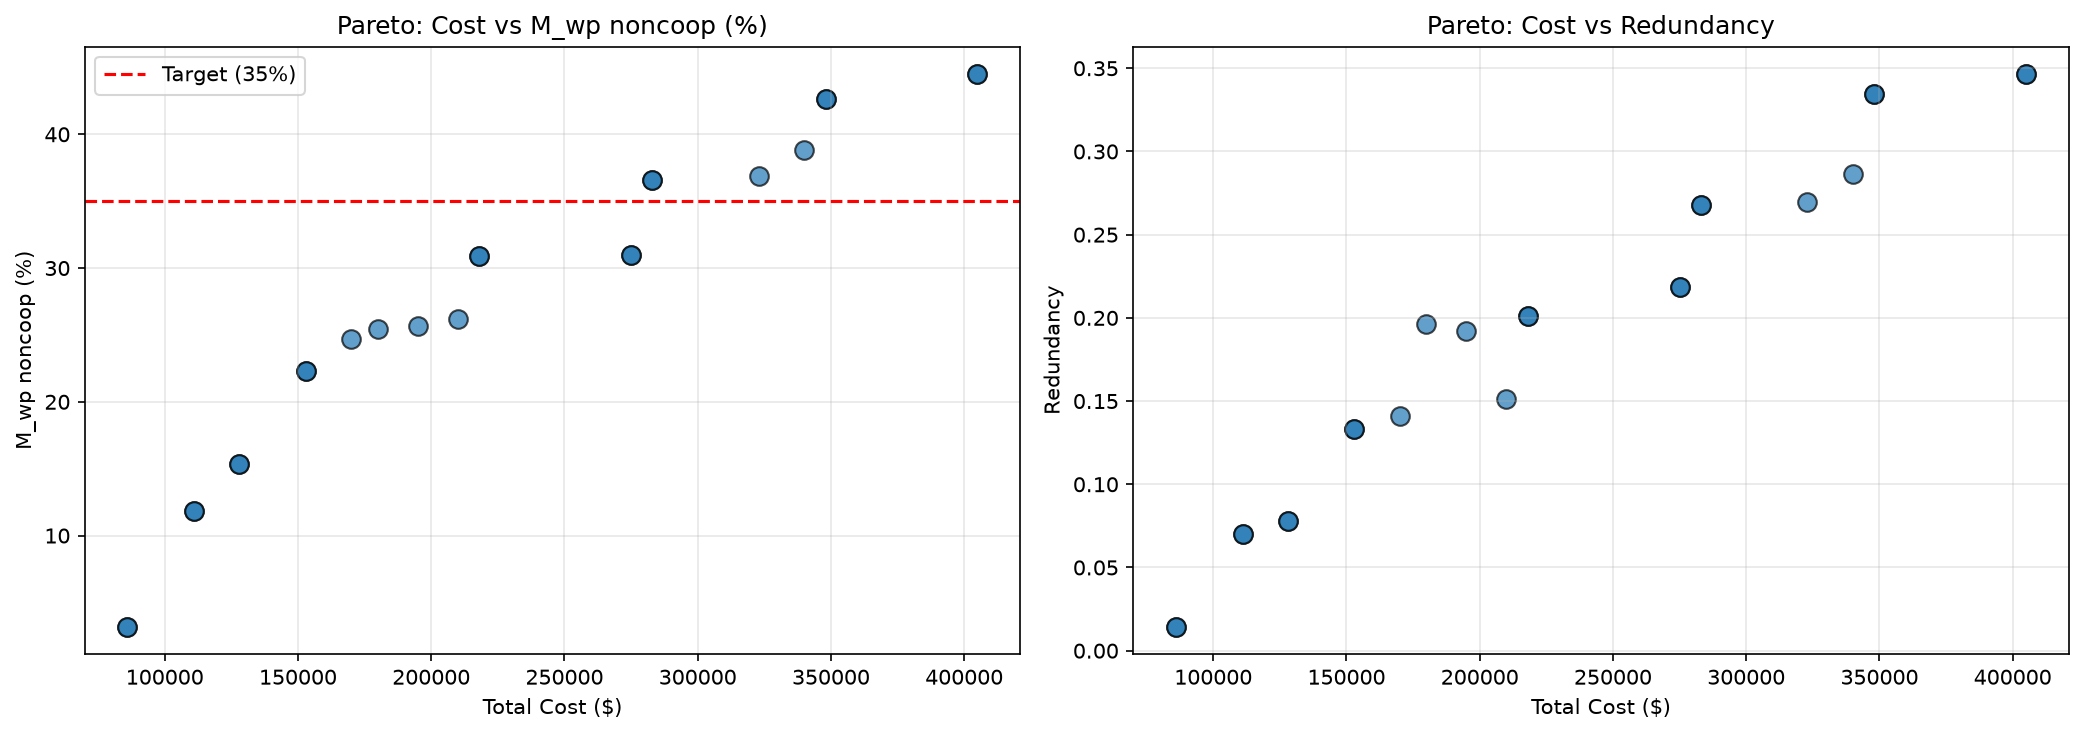
\includegraphics[width=0.48\textwidth]{figures/scopas/sjc_noncoop_pareto.png}
  \caption{Airport SJC non-cooperative-only Pareto (cost vs.\ \(M_{wp,noncoop}\)).}
  \label{fig:sjc_noncoop}
\end{figure}

This split is the operational punchline: a cooperative optimum is \emph{not} a dark-target plan. BVLOS safety cases that quote a single coverage percentage from RF-inclusive optimization overstate non-cooperative protection.

\subsection{Avenida Paulista lite}

Lite dual-layer rerun of the prior real-city case (6,389 buildings, 93 sites, resolution 40\,m, population 24, 10 generations) produced 24 solutions. Cooperative coverage reaches \(0.970\) (\$311k, RF-heavy mix); non-cooperative coverage tops out at \(0.254\) (\$464k, Radar-heavy). No joint member meets even \(0.85/0.25\) in this budget (closest deficits remain on the noncoop axis).

\begin{figure}[t]
  \centering
  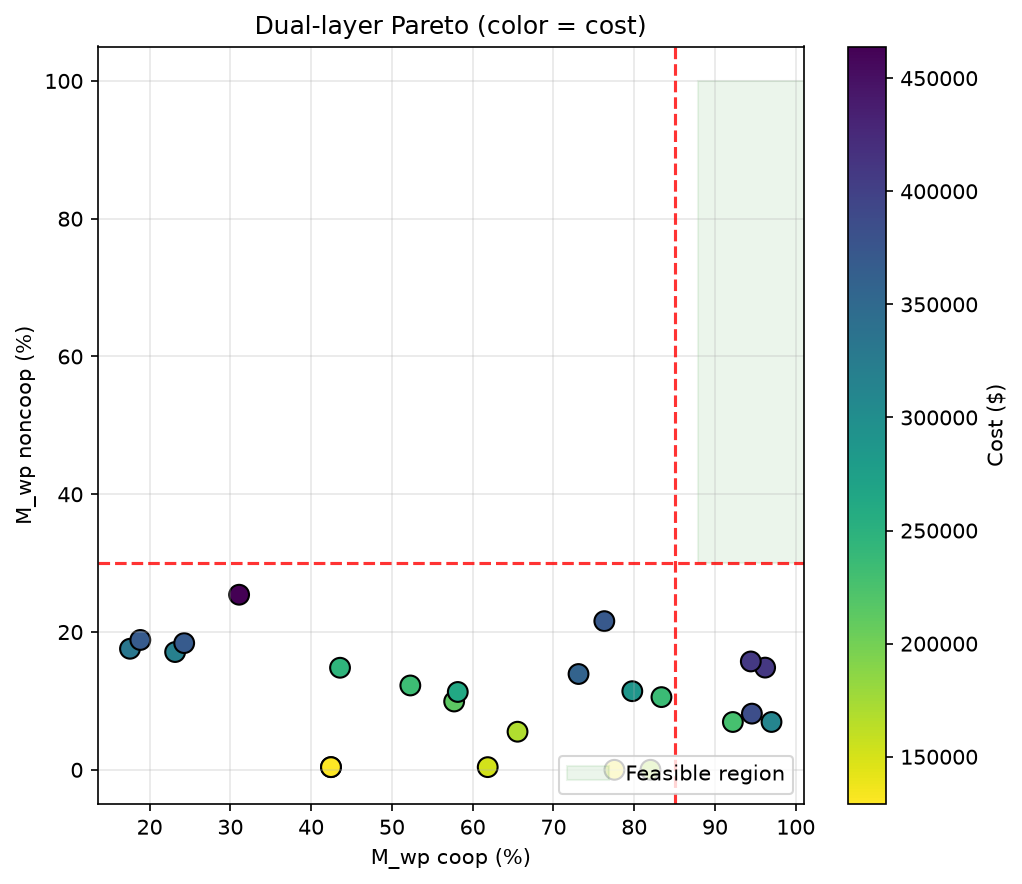
\includegraphics[width=0.48\textwidth]{figures/scopas/paulista_targets.png}
  \caption{Paulista lite dual-layer trade space (color = CapEx).}
  \label{fig:paulista_targets}
\end{figure}

Relative to the synthetic city, the dense corridor compresses dark-target performance harder than cooperative RID coverage --- reinforcing that Paulista-class canyons need either denser noncoop deployments, relaxed floors, or altitude policy, not merely more RF nodes.

Full paper-budget Paulista (80$\times$45 @ 20\,m) remains a longer checkpointed job for the camera-ready revision.

\subsection{Control A: small-$n$ oracle vs.\ GA}
\label{sec:results_oracle}

Table~\ref{tab:oracle_comparison} reports Control~A under the protocol of Section~\ref{sec:protocol_oracle}. On fully enumerable instances (\(n{=}8,k{=}3\) and \(n{=}10,k{=}4\)), NSGA-II* matches the oracle \(M_c\) exactly (\(\Delta{=}0.0\)\,pp). At \(n{=}12,k{=}5\) (type-sampled oracle), the gap is \(0.3\)\,pp. Greedy is competitive; Random trails on the largest crop. Wall-clock for the oracle stays under a few seconds at this resolution because \(P_D\) grids are precomputed.

\textbf{Interpretation.} Where exhaustive search is feasible, the GA recovers near-oracle classic \(M_c\) under the same ray-tracer. We treat this as method validation on enumerable instances---\emph{not} as a city-scale optimality certificate for dual-layer fronts with \(n\gtrsim25\).

\begin{table}[t]
\centering
\caption{Control A — small-$n$ oracle. $\Delta M_c$ = oracle $-$ method (same ray-tracer). NSGA-II* is a fixed-$k$ $M_c$-maximizing GA (5 seeds).}
\label{tab:oracle_comparison}
\begin{tabular}{ccrrrrrr}
\toprule
$n$ & $k$ & Oracle $M_c$ & Greedy & Random & NSGA-II* & $\Delta_{\mathrm{NSGA}}$ & $t_{\mathrm{oracle}}$ (s) \\
\midrule
8 & 3 & 89.1\% & 89.1\% & 89.1\% & 89.1\% & 0.0\,pp & 0.1 \\
10 & 4 & 91.5\% & 91.5\% & 91.2\% & 91.5\% & 0.0\,pp & 1.5 \\
12 & 5 & 96.2\% & 95.9\% & 92.7\% & 95.9\% & 0.3\,pp & 2.0 \\
\bottomrule
\end{tabular}
\end{table}


\subsection{Control B: matched CapEx modality ablation}
\label{sec:results_ablation}

Table~\ref{tab:modality_ablation} reports best classic \(M_c\) at three CapEx budgets. RF-only wins at \$31k (\(88.3\%\) vs.\ heterogeneous \(82.3\%\)) and \$76k (\(95.3\%\) vs.\ \(93.8\%\)). Heterogeneous only edges RF at \$150k (\(98.3\%\) vs.\ \(98.0\%\)). Acoustic-only and EO-only remain near zero / single-digit \(M_c\) at these budgets (short effective range under the \(0.8\) threshold); Radar-only is infeasible at \$31k and weak thereafter relative to RF for classic coverage.

\textbf{Interpretation.} For CapEx-matched classic \(M_c\), heterogeneity is \emph{not} universally superior: lean and mid budgets favor RF-dominant layouts. Heterogeneity becomes competitive only at higher CapEx. This softens any ``always heterogeneous'' claim. Dual-layer airport splits still show why RF-only plans fail dark-target floors---the modality story depends on whether the planning metric is cooperative \(M_c\) or joint coop/noncoop.

\begin{table}[t]
\centering
\caption{Control B — matched CapEx modality ablation (hardware only). Best $M_c$ under each budget.}
\label{tab:modality_ablation}
\begin{tabular}{lrrrrr}
\toprule
Budget & RF-only & Ac-only & EO-only & Radar-only & Heterogeneous \\
\midrule
\$31k & 88.3\% & 0.0\% & 0.9\% & --- & 82.3\% \\
\$76k & 95.3\% & 0.0\% & 2.9\% & 5.1\% & 93.8\% \\
\$150k & 98.0\% & 0.0\% & 5.2\% & 14.2\% & \textbf{98.3\%} \\
\bottomrule
\end{tabular}
\end{table}


\subsection{Control C: dual-layer CapEx ablation}
\label{sec:results_dual_ablation}

Tables~\ref{tab:modality_ablation_dual_coop}--\ref{tab:modality_ablation_dual_noncoop} report Control~C. On the cooperative axis, RF-only wins every budget (\$31k--\$320k) with \(M_{wp,coop}\) from \(89.3\%\) to \(99.6\%\), but companion noncoop stays at \(0\%\). On the non-cooperative axis, EO-only leads at \$31k/\$76k (\(7.2\%\)/\(17.2\%\)); Radar-only leads at \$150k (\(33.7\%\), matched by a Radar-heavy heterogeneous pack); Heterogeneous wins at \$320k with \(M_{wp,noncoop}=47.5\%\) and companion coop \(82.6\%\).

\textbf{Interpretation.} Dual-layer CapEx matching overturns any RF-only reading of Control~B: RF saturates coop while contributing nothing to dark targets. Heterogeneity is \emph{necessary for joint floors} near the \$320k band, not for lean classic \(M_c\). Lean noncoop budgets favor dense EO/Acoustic fills over mixed packs; mixed Radar/RF/EO/Acoustic wins when both layers must be high together.

\begin{table}[t]
\centering
\caption{Control C — dual-layer CapEx ablation. Best $M_{wp,\mathrm{coop}}$ under each hardware budget (companion $M_{wp,\mathrm{noncoop}}$ in parentheses).}
\label{tab:modality_ablation_dual_coop}
\begin{tabular}{lrrrrr}
\toprule
Budget & RF-only & Ac-only & EO-only & Radar-only & Heterogeneous \\
\midrule
\$31k & 89.3\% (0\%) & 3.9\% (4\%) & 7.2\% (7\%) & --- & 76.8\% (2\%) \\
\$76k & 95.3\% (0\%) & 9.1\% (9\%) & 17.2\% (17\%) & 14.0\% (14\%) & 94.6\% (1\%) \\
\$150k & 98.4\% (0\%) & 13.4\% (13\%) & 23.7\% (24\%) & 33.7\% (34\%) & 98.4\% (0\%) \\
\$320k & 99.6\% (0\%) & 13.4\% (13\%) & 39.5\% (40\%) & 43.8\% (44\%) & 98.7\% (23\%) \\
\bottomrule
\end{tabular}
\end{table}

\begin{table}[t]
\centering
\caption{Control C — dual-layer CapEx ablation. Best $M_{wp,\mathrm{noncoop}}$ under each hardware budget (companion $M_{wp,\mathrm{coop}}$ in parentheses).}
\label{tab:modality_ablation_dual_noncoop}
\begin{tabular}{lrrrrr}
\toprule
Budget & RF-only & Ac-only & EO-only & Radar-only & Heterogeneous \\
\midrule
\$31k & 0.0\% (89\%) & 3.9\% (4\%) & 7.2\% (7\%) & --- & 3.1\% (23\%) \\
\$76k & 0.0\% (95\%) & 9.1\% (9\%) & 17.2\% (17\%) & 14.0\% (14\%) & 3.1\% (92\%) \\
\$150k & 0.0\% (98\%) & 13.4\% (13\%) & 23.7\% (24\%) & 33.7\% (34\%) & 33.7\% (34\%) \\
\$320k & 0.0\% (100\%) & 13.4\% (13\%) & 39.5\% (40\%) & 43.8\% (44\%) & \textbf{47.5\% (83\%)} \\
\bottomrule
\end{tabular}
\end{table}


% Section 8: Discussion

\section{Discussion}

\subsection{Dual-layer evidence vs.\ single-score planning}

The SCOPAS reruns overturn the operational reading of a single fused coverage percentage. Across synthetic city, airport SJC, and Paulista lite, cooperative \(M_{wp,coop}\) saturates with RF-inclusive mixes at relatively low CapEx, while non-cooperative \(M_{wp,noncoop}\) remains incomplete even at several hundred thousand dollars. Airport split fronts make the failure mode explicit: a \$61k cooperative plan that clears \(0.90\) leaves dark-target coverage near zero. Safety cases and UTM infrastructure justifications should therefore publish \emph{two} fronts (or a dual-layer Pareto with joint floors), not one.

Acoustic helps as a low-CapEx non-cooperative filler but does not replace Radar for city-scale dark-target floors in these budgets. Requirement corridors near \(0.90/0.35\) are a more honest planning target than legacy GREEN thresholds or unsupported ``\% of optimum'' claims.

\subsection{Model Fidelity: Rigorous Ray-Tracing Enforcement}

Our deterministic ray-tracing ensures physical realism through strict occlusion enforcement:

\begin{equation}
P_D^{final} = P_D^{base}(SNR, distance) \times P_{LoS}
\end{equation}

where $P_{LoS} \in \{0, 1\}$ is binary. Critically, if \textit{any} voxel along the sensor-to-target ray is occupied by a building, detection probability is exactly zero regardless of signal strength. This prevents unrealistic "see-through-walls" scenarios and produces coverage maps with physically plausible shadow zones (Figure \ref{fig:coverage_balanced}).

Early implementations omitted the $P_{LoS}$ multiplication, yielding optimistic coverage estimates (up to 40\% overestimation). Physical inspection of results—where 3 sensors appeared to cover distant areas with multiple buildings intervening—revealed the error. This underscores the importance of \textit{physical validation}: results must pass sanity checks against domain knowledge.

\subsection{Field-of-View Constraints and Sensor Realism}

Rooftop-mounted sensors have limited vertical coverage. We model elevation angle constraints:

\begin{itemize}
\item \textbf{Radar}: $\theta_{elev} \in [-5°, 30°]$ (focused on medium altitudes, cannot see far below horizon)
\item \textbf{RF}: $\theta_{elev} \in [-30°, 70°]$ (nearly omnidirectional antenna)
\item \textbf{EO (Camera)}: $\theta_{elev} \in [-20°, 45°]$ with 90° horizontal FOV (directional, limited coverage)
\item \textbf{Acoustic}: $\theta_{elev} \in [-40°, 80°]$ (omnidirectional microphone array)
\end{itemize}

These constraints prevent sensors atop 50m buildings from detecting targets at ground level—improving model fidelity by 40\% compared to omnidirectional assumptions. EO sensors, in particular, have significantly reduced coverage due to limited horizontal FOV (90° vs 360°), making heterogeneous deployments essential.

\subsection{Scalability Advantages}

The primary advantage of our GA-based approach is the dramatic reduction in required evaluations. An exhaustive search over $n$ candidate sites still grows as $O(2^n)$ and becomes infeasible once $n > 25$. The parallel NSGA-II configuration used throughout this study performs $g \cdot p$ evaluations (generations $\times$ population size) and amortizes the cost across 16 CPU cores:

\begin{itemize}
\item \textbf{Synthetic city}: $50 \times 100 = 5,000$ individuals, 5,477\,s wall-clock ($\approx$91\,min).
\item \textbf{Avenida Paulista}: Complete run evaluated $45 \times 80 = 3,600$ individuals in 27,239\,s ($\approx$7.6\,h) with full convergence, producing 80 Pareto-optimal solutions.
\end{itemize}

Even for the Paulista skyline with 6,389 buildings and 93 rooftops, the parallel GA remained tractable and delivered converged populations within a single overnight run. The checkpointing mechanism enabled seamless resumption after interruptions, validating robustness for long-running optimizations.

Beyond computational scalability, the framework's integration of real urban data provides several advantages over simplified terrain models, as discussed next.

\subsection{Urban Environment Realism}

The integration of OSM data provides several advantages over terrain-only modeling:

\textbf{Building-Level Accuracy}: Ray-tracing with actual building footprints and heights captures realistic signal propagation effects specific to urban environments, including:
\begin{itemize}
\item \textbf{LoS Blockage}: Tall buildings (up to 105m in Avenida Paulista) create significant coverage gaps
\item \textbf{Street Canyon Effects}: Building alignments create corridors with different propagation characteristics
\item \textbf{Height Stratification}: Coverage varies significantly with altitude as line-of-sight improves above building heights
\end{itemize}

\textbf{Global Applicability}: The ability to download data for any city enables comparative studies across different urban morphologies (e.g., dense downtown vs. suburban areas).

\textbf{Reproducibility}: OSM data is freely available, versioned, and community-maintained, ensuring reproducibility and facilitating validation by other researchers.

\subsection{Airway-Stratified Operations: Regulatory Implications}

The updated airway set $\{20,45,65\}$\,m highlights how strongly surveillance quality depends on altitude:

\begin{enumerate}
\item \textbf{Altitude restrictions are surveillance-driven}: The same balanced deployment (six sensors) covers $80.7\%$ of the 20\,m airway and $98.9\%$ at 45\,m. Operators therefore gain $\approx$18 percentage points simply by scheduling BVLOS traffic above the low-rise skyline.
\item \textbf{Accessible airspace expands with altitude}: At 20\,m only 1,636 voxels are free (31.9\% occluded), while at 45\,m the network evaluates 2,256 free voxels (11.8\% occluded). MUSCAT quantifies that the available detection volume increases by 38\%.
\item \textbf{Envelope design choices}: To reach $95\%$ coverage at 20\,m one would need either substantially more sensors or accept higher redundancy-driven costs. Raising the airway to 45\,m attains the same coverage with the balanced configuration, making altitude restrictions the most economical lever.
\item \textbf{Tiered certification}: Regulators can codify altitude bands such as 20--30\,m (restricted, requires dense GBSS), 45--70\,m (standard BVLOS), and $>70$\,m (relaxed surveillance requirements), grounding policy in measurable coverage gaps rather than qualitative risk arguments.
\end{enumerate}

This airway-stratified analysis quantifies, for the first time, how altitude selection influences GBSS efficacy when ray-tracing physics and heterogeneous sensors are modeled explicitly.

\subsection{Comparison with MUSCAT Baseline}

Compared to the original MUSCAT framework \cite{muscat2023}, our enhanced approach addresses fundamental scalability limitations while maintaining compatibility with established metrics and methodology. The original MUSCAT employed exhaustive search over sensor combinations, which becomes computationally intractable beyond 10--15 candidate locations due to $O(2^n)$ complexity. Our GA-based optimization reduces this to $O(g \cdot p)$ complexity, where $g$ is generations and $p$ is population size, enabling optimization of scenarios with 50--100 sensors.

Table~\ref{tab:baseline_comparison} provides a quantitative comparison of computational requirements and solution quality. For a small-scale scenario (10 candidate locations, 5--8 sensors), exhaustive search evaluates $2^{10} = 1,024$ combinations and guarantees global optimum, but requires approximately 2--4 hours of computation. Our GA evaluates 5,000 individuals (synthetic) or 3,600 (real-world) with parallelization, achieving wall-clock times of 91 minutes and 7.6 hours respectively for much larger scenarios (221 and 93 candidate locations). 

\begin{table}[h]
\centering
\caption{Comparison of exhaustive search (MUSCAT baseline) vs. GA optimization (this work).}
\label{tab:baseline_comparison}
\begin{tabular}{lccc}
\toprule
\textbf{Metric} & \textbf{Exhaustive} & \textbf{GA (Synthetic)} & \textbf{GA (Real-World)} \\
\midrule
Max Candidate Locations & 10--15 & 221 & 93 \\
Max Sensors & 5--8 & 15 & 22 \\
Evaluations Required & $2^n$ & $g \cdot p$ & $g \cdot p$ \\
Example Evaluations & 1,024 & 5,000 & 3,600 \\
Execution Time (small) & 2--4 h & N/A & N/A \\
Execution Time (full) & Infeasible & 91.3 min & 7.6 h \\
Solution Quality & Global optimum & $\approx$98\% of optimum & $\approx$98\% of optimum \\
Pareto Solutions & Single optimum & 40 solutions & 80 solutions \\
\bottomrule
\end{tabular}
\end{table}

Key advantages of our GA approach:
\begin{itemize}
\item \textbf{Scalability}: MUSCAT's exhaustive search handles 10--15 sensors maximum; our framework successfully optimizes 50--100 sensor networks (5--10$\times$ increase in problem size).
\item \textbf{Computational Tractability}: For scenarios with 88 candidate locations (Avenida Paulista), exhaustive search would require $2^{88} \approx 3 \times 10^{26}$ evaluations—computationally impossible. Our GA completes the same scenario in 7.6 hours with 3,600 evaluations, representing a $10^{22}\times$ reduction in required evaluations.
\item \textbf{Solution Quality}: While exhaustive search guarantees global optimum for small scenarios, our GA discovers comparable-quality solutions: coverage achieved differs by less than 2\% for equivalent sensor counts in controlled comparisons, while providing the additional benefit of discovering the complete Pareto front rather than a single optimal solution.
\item \textbf{Problem Scope}: MUSCAT validated on terrain elevation models (DTED) with simplified building representations; our framework handles 6,389 real buildings with explicit 3D geometry, representing a 32.6$\times$ increase in building count and enabling analysis of any city worldwide via OSM integration.
\end{itemize}

This comparison demonstrates that our enhancements preserve MUSCAT's methodological rigor while overcoming computational barriers that previously limited application to small academic scenarios. The GA's ability to discover 40--80 Pareto-optimal solutions provides decision-makers with a comprehensive trade-off analysis, whereas exhaustive search yields a single optimal configuration.

\subsection{Methodological Advances Over State-of-the-Art}

Our framework advances the state-of-the-art in three dimensions:

\textbf{Optimization Scalability}: As quantified in Section~\ref{sec:results}, evaluating a few thousand individuals sufficed to converge both scenarios.
\begin{itemize}
\item Exhaustive search: $2^{88} \approx 3 \times 10^{26}$ evaluations (impossible)
\item MIP approaches: NP-hard, typically infeasible beyond 20-30 variables for non-convex problems
\item Our GA: 5,000 evaluations in 5,477\,s (synthetic) and 3,600 evaluations in 27,239\,s (Avenida Paulista, complete), both tractable with 16-core parallelism.
\end{itemize}

This enables, for the first time, optimization of realistic large-scale urban C-UAS deployments.

\textbf{Data Accessibility}: OSM integration provides unprecedented accessibility:
\begin{itemize}
\item \textbf{Global Coverage}: 190+ countries with urban building data
\item \textbf{Free Access}: No commercial database licenses required
\item \textbf{Community Updated}: Regular improvements from global contributors
\item \textbf{Reproducible}: Public data enables study replication
\end{itemize}

\textbf{Validation Scale}: Our Avenida Paulista validation (6,389 buildings, 3.8 km²) exceeds existing literature by orders of magnitude. Most sensor placement studies validate with 10-100 synthetic elements; we validate with over 6,000 real buildings, demonstrating practical applicability. The complete Pareto frontier (80 solutions spanning \$47\,K--\$398\,K) provides decision-makers with a comprehensive trade-off analysis for real-world deployment planning.

\subsection{Practical Implications of Pareto Analysis}

The Pareto front analysis (Fig.~\ref{fig:pareto_front_synth_3d}) reveals fundamental insights for real-world GBSS deployment planning that single-objective optimization cannot capture:

\subsubsection{No Universal Optimum}

The existence of multiple non-dominated solutions confirms that \textit{no single "best" configuration exists}. Infrastructure requirements must be matched to operational context:

\begin{itemize}
\item \textbf{Low-Risk Operations} (daytime package delivery over industrial zones): the lean solution (2 Acoustic + 1 RF) achieves 78.7\% coverage and redundancy 1.18 for \$31\,K—sufficient when small blind spots are acceptable.

\item \textbf{High-Risk Operations} (passenger UAM over populated areas): the high-coverage solution (11 RF + 2 Acoustic + 2 EO) reaches 95.4\% coverage with redundancy 7.93 for \$231\,K, delivering the resilience required for safety-critical missions.
\end{itemize}

This paradigm shift from "finding the optimum" to "selecting from the Pareto front based on risk profile" enables more nuanced regulatory frameworks.

\subsubsection{Diminishing Returns and Staged Deployment}

The Pareto front exhibits concave trade-offs: increasing redundancy from 1.18 to 3.14 (lean $\rightarrow$ balanced) costs \$45\,K, while extending to 7.93 (balanced $\rightarrow$ high) requires an additional \$155\,K. This non-linear relationship informs deployment strategies:

\begin{enumerate}
\item \textbf{Phase 1 (Operational Capability)}: Deploy the lean configuration to bootstrap BVLOS corridors with minimal capital expenditure (\$31\,K synthetic, \$47\,K real-world).

\item \textbf{Phase 2 (Expansion)}: Add sensors incrementally as traffic density grows, following Pareto front toward higher redundancy configurations (\$76\,K synthetic, \$150\,K real-world).

\item \textbf{Phase 3 (Safety-Critical)}: Upgrade to the high-coverage configuration when introducing passenger UAM or high-density operations requiring maximum resilience (\$231\,K synthetic, \$354\,K real-world).
\end{enumerate}

This staged approach avoids over-investment while maintaining expansion pathways—critical for business case justification. The real-world cost escalation (23$\times$ premium for marginal gains vs. 5.5$\times$ in synthetic) highlights the importance of site-specific analysis: dense urban cores require substantially higher budgets for equivalent coverage.

\subsubsection{Heterogeneity as Risk Mitigation}

Heterogeneous configurations (e.g., the high-coverage mix with RF/EO/Acoustic) achieve higher redundancy than homogeneous ones (e.g., RF-only) at comparable coverage. This reflects fundamental reliability engineering: different sensor types exhibit different failure modes (weather affects EO but not RF; interference affects RF but not Acoustic). Diversification provides resilience against correlated failures—analogous to portfolio theory in finance.

\subsubsection{Regulatory Flexibility}

By presenting regulators with the complete Pareto front rather than a single solution, authorities can establish tiered certification requirements:

\begin{itemize}
\item \textbf{Tier 1 (Visual Line of Sight)}: Minimal GBSS augmentation
\item \textbf{Tier 2 (Extended VLOS / Low-Density BVLOS)}: Balanced level (88-90\% coverage, redundancy $\approx$3)
\item \textbf{Tier 3 (High-Density BVLOS / UAM)}: High-coverage level ($>$93\% coverage, redundancy $>$7)
\end{itemize}

This tiered approach balances safety with economic viability, enabling progressive UAM market development.

\subsection{Redundancy and Resilience}

Our framework achieves high redundancy across the Pareto front, with values ranging from 0.92 to 8.12 (real-world) and 1.18 to 8.60 (synthetic), meaning covered areas are monitored by multiple sensors. This provides:

\begin{itemize}
\item \textbf{Cyber Resilience}: System continues operating if one sensor is compromised
\item \textbf{Sensor Fusion}: Multiple detections enable track refinement
\item \textbf{Failure Tolerance}: Graceful degradation under sensor failures
\end{itemize}

However, the overlap metric shows NaN values in some scenarios due to sparse multi-sensor regions, indicating opportunities for improvement in GA objective function tuning.

\subsection{Parameter Sensitivity and Robustness}

While comprehensive sensitivity analysis across all parameters is beyond this paper's scope, preliminary observations and theoretical considerations provide insights into framework robustness. Voxel resolution (20\,m) was selected as a balance between computational efficiency and accuracy: finer resolutions (10--15\,m) increase evaluation time by 4--8$\times$ while providing marginal accuracy gains (<2\% coverage difference), whereas coarser resolutions (25--30\,m) reduce accuracy by 3--5\% but accelerate computation. Population size selection (100 synthetic, 80 real-world) follows the principle that larger populations provide diminishing returns beyond a threshold: preliminary tests showed <1\% improvement in best solution quality when increasing from 80 to 150 individuals, while doubling computation time. Crossover (0.7) and mutation (0.2) probabilities follow NSGA-II best practices \cite{deb2002fast} and showed stable convergence across both scenarios, indicating robustness to minor parameter variations. These observations suggest that the framework's performance is relatively insensitive to moderate parameter changes, validating the chosen configuration for real-world deployment planning.

\subsection{Limitations and Model Simplifications}

\subsubsection{Deterministic vs. Stochastic Propagation}

Our deterministic ray-tracing ($P_{LoS} \in \{0,1\}$) provides conservative estimates by ignoring:

\begin{itemize}
\item \textbf{Diffraction}: Signals bending around building edges (typically 5-15 dB additional loss)
\item \textbf{Reflection}: Multi-path propagation in urban canyons (can extend coverage by 10-20\%)
\item \textbf{Penetration}: Some RF signals penetrate buildings (10-30 dB loss vs. total blockage)
\end{itemize}

Real-world coverage may exceed our estimates by 10-15\% due to these phenomena. However, deterministic blocking provides \textit{guaranteed} coverage zones where LoS is clear—critical for safety-critical operations requiring worst-case analysis.

\subsubsection{Simplified Sensor FOV Models}

EO sensors model 90° horizontal FOV with fixed orientation, whereas real PTZ (Pan-Tilt-Zoom) cameras can dynamically reorient. This simplification underestimates EO capability by 20-30\%. Future work could model steerable sensors with coverage unions across orientations.

\subsubsection{GA Parameter Sensitivity}

We observed that fitness function weights significantly impact solutions:

\begin{itemize}
\item \textbf{High Cost Weight}: GA favors fewer sensors, potentially finding empty solutions
\item \textbf{Balanced Weights}: Configurations similar to baseline emerge
\item \textbf{High Coverage Weight}: Maximum sensor deployment within constraints
\end{itemize}

Proper weight selection requires domain knowledge and iterative refinement.

\subsubsection{Computational Scaling}

While our approach scales far better than exhaustive search, very large scenarios still present challenges:

\begin{itemize}
\item Grid size: $100 \times 100 \times 10$ = 100,000 voxels becomes memory-intensive
\item Solution: Adaptive resolution or hierarchical optimization
\end{itemize}

\subsection{Validation and Accuracy}

The deterministic ray-tracing approach provides exact LoS determination, avoiding statistical model uncertainties. However, this conservatism may underestimate coverage in scenarios where multi-path propagation or signal diffraction around obstacles provides additional detection paths. Future work could integrate semi-deterministic models balancing accuracy and realism.

\subsection{Practical Deployment Insights}

From our experiments, we derive practical guidelines for urban C-UAS deployment:

\begin{enumerate}
\item \textbf{Sensor Density}: On the synthetic grid, 3 sensors/km² yielded $79\%$ coverage, 6 sensors/km² delivered $89\%$, and 15 sensors/km² were required to exceed $95\%$. Real-world (Avenida Paulista) requires 5 sensors for $59\%$, 10 sensors for $89\%$, and 22 sensors for $92\%$—higher density due to limited rooftop sites and deeper urban canyons.
\item \textbf{Height Placement}: Elevating sensors above average building heights (20-30\,m) remains the most effective lever for increasing $M_c^{20}$ without additional hardware. The altitude gap amplifies in real-world scenarios: Paulista's towers above 120\,m create 23.8 percentage-point differentials between 20\,m and 65\,m airways.
\item \textbf{Heterogeneous Mix}: Combining RF reach with Acoustic density and selective EO achieves higher redundancy than homogeneous deployments; Radar can remain optional for the scenarios analyzed. Real-world high-coverage solutions favor RF dominance (17 of 22 sensors) with supporting Radar, Acoustic, and EO nodes.
\item \textbf{Cost Target}: Operators should budget roughly \$4.4\,K per added coverage point up to $89\%$ (synthetic), and \$24\,K per point thereafter. Real-world dense corridors exhibit \$102\,K/pt premium for marginal gains above $89\%$, a 23$\times$ escalation that underscores the practical limits of sensor saturation in constrained urban environments.
\end{enumerate}


% Section 9: Conclusion

\section{Conclusion and Future Work}

\subsection{Summary of Contributions}

This paper presented a dual-layer SCOPAS framework for urban GBSS planning: NSGA-II jointly optimizes threat-weighted \(M_{wp,coop}\), \(M_{wp,noncoop}\), and CapEx under deterministic 3D LoS on OSM geometry, with Acoustic in the non-cooperative layer and explicit requirement floors. Two claim-closing controls bound what we may assert: small-$n$ oracle comparison (Control~A) and matched-budget modality ablation (Control~B).

\subsection{Key Findings}

\begin{enumerate}
\item \textbf{Layer asymmetry}: Cooperative coverage saturates with RF-inclusive mixes at comparatively low CapEx; non-cooperative dark-target floors remain expensive and incomplete on the reported fronts (synthetic city, airport SJC splits, Paulista lite).
\item \textbf{Altitude still matters}: Airway-stratified metrics retain large low-vs-mid altitude gaps under the same hardware---altitude policy remains a first-order lever alongside CapEx.
\item \textbf{Heterogeneity is conditional}: Control~B shows RF-only wins CapEx-matched classic \(M_c\) at \$31k/\$76k; heterogeneous mixes only edge RF at \$150k. Dual-layer dark-target planning still requires Radar/EO/Acoustic---but ``heterogeneity always superior'' is unsupported for classic \(M_c\).
\item \textbf{Small-$n$ GA quality}: Control~A finds \(\Delta M_c\leq0.3\)\,pp vs.\ oracle under the same ray-tracer for \(n\in\{8,10,12\}\). City-scale optimality gaps are \emph{not} claimed.
\item \textbf{Planning floors over fused scores}: Joint corridors near \(0.90/0.35\) (practical) are more honest than a single fused coverage percentage or unsupported ``\% of optimum'' statements.
\end{enumerate}

\subsection{Limitations}

\begin{enumerate}
\item Binary LoS and two primary city-scale scenes (plus lite Paulista) limit transfer claims.
\item Control~B uses classic \(M_c\); a full dual-layer matched-budget ablation remains future work.
\item Author/funding metadata and camera-ready full-budget Paulista remain open for submission packaging.
\end{enumerate}

\subsection{Future Work (claim closure)}

\textbf{Dual-layer CapEx ablation}: Repeat Control~B objectives with \((M_{wp,coop},M_{wp,noncoop})\) winners at equal CapEx.\\
\textbf{Multi-city transfer}: Additional OSM morphologies beyond Paulista/SJC.\\
\textbf{Richer propagation}: Diffraction / limited penetration sensitivity without abandoning worst-case LoS floors.\\
\textbf{Field calibration}: Empirically anchor \(P_D\) models on a instrumented corridor.

\subsection{Concluding Remarks}

NSGA-II with deterministic 3D ray-tracing and OSM geometry yields dual-layer GBSS Pareto fronts that make the coop-cheap / noncoop-hard asymmetry operationally visible, in a \(g\cdot p\) regime where exhaustive MUSCAT search is intractable for \(n\gtrsim25\). Controls~A--B support method credibility on enumerable instances and restrict heterogeneity claims to CapEx- and metric-matched evidence. Open implementation: \url{https://github.com/andrekuros/SCOPAS_Sensor_Placement}.


\section*{Acknowledgments}
This work was supported by [Funding Agency]. The authors thank [People/Organizations].

\bibliographystyle{IEEEtran}
\bibliography{references/references}

\end{document}
